\documentclass{beamer}
%\usepackage[margin=1in]{geometry}
\usepackage{amsthm,amsmath,amsfonts,hyperref,graphicx,color,multicol}
\usepackage{enumitem,tikz}

%%%%%%%%%%
%Beamer Template Customization
%%%%%%%%%%
\setbeamertemplate{navigation symbols}{}
\setbeamertemplate{theorems}[ams style]
\setbeamertemplate{blocks}[rounded]

\definecolor{Blu}{RGB}{43,62,133} % UWEC Blue
\setbeamercolor{structure}{fg=Blu} % Titles

%Unnumbered footnotes:
\newcommand{\blfootnote}[1]{%
	\begingroup
	\renewcommand\thefootnote{}\footnote{#1}%
	\addtocounter{footnote}{-1}%
	\endgroup
}


%%%%%%%%%%
%Custom Commands
%%%%%%%%%%
\newcommand{\R}{\mathbb{R}}
\newcommand{\veca}{\vec{a}}
\newcommand{\vecb}{\vec{b}}
\newcommand{\vece}{\vec{e}}
\newcommand{\vecu}{\vec{u}}
\newcommand{\vecv}{\vec{v}}
\newcommand{\vecw}{\vec{w}}
\newcommand{\vecx}{\vec{x}}
\newcommand{\zerovector}{\vec{0}}

\newcommand{\ds}{\displaystyle}

\newcommand{\fn}{\insertframenumber}

\newcommand{\rank}{\operatorname{rank}}
\newcommand{\adj}{\operatorname{adj}}

\newcommand{\blank}[1]{\underline{\hspace*{#1}}}


%%%%%%%%%%
%Custom Theorem Environments
%%%%%%%%%%
\theoremstyle{definition}
\newtheorem{exercise}{Exercise}
\newtheorem{question}[exercise]{Question}
\newtheorem*{defn}{Definition}
\newtheorem*{exa}{Example}
\newtheorem*{disc}{Group Discussion}
\newtheorem*{nb}{Note}
\newtheorem*{recall}{Recall}
\renewcommand{\emph}[1]{{\color{blue}\texttt{#1}}}

\definecolor{Gold}{RGB}{237, 172, 26}
%Statement block
\newenvironment{statementblock}[1]{%
	\setbeamercolor{block body}{bg=Gold!20}
	\setbeamercolor{block title}{bg=Gold}
	\begin{block}{\textbf{#1.}}}{\end{block}}





\begin{document}
	\title{Math 324: Linear Algebra}
	\subtitle{Section 4.3: Subspaces of Vector Spaces}
	\author{Mckenzie West}
	\date{Last Updated: \today}
\begin{frame}
\maketitle
\end{frame}

\begin{frame}{\insertframenumber}
	\begin{block}{\textbf{Last Time.}}
	\begin{itemize}[label=--]
		\item Proving Something is not a Vector Space
		\item Definition of Subspaces
		\item Test for Subspaces
	\end{itemize}
	\end{block}
	\begin{block}{\textbf{Today.}}
		\begin{itemize}[label=--]
			\item Subspaces of $\R^2$
			\item Subspaces of $\R^3$
			\item Intersections of Subspaces
		\end{itemize}
	\end{block}
\end{frame}
\begin{frame}{\fn}
	\begin{exercise}
		Solve the homogeneous system of equations with coefficient matrix \[A=\begin{bmatrix}1&4&7\\2&5&8\\3&6&9\end{bmatrix}.\]
	
	Is the set of solutions to this system a vector space with standard operations from $\R^3$?
	\end{exercise}
	\begin{exercise}
		Let $A=\begin{bmatrix}1&3\\1&3\end{bmatrix}$ and $\vec b=\begin{bmatrix}-1\\-1\end{bmatrix}$.  Is the set of solutions to the system $A\vec x=\vec b$ a vector space with the standard operations in $\R^2$?
	\end{exercise}
\end{frame}
\begin{frame}{\fn}
\begin{exercise}
	Let $A$ be any $n\times n$ matrix.  Complete the proof of the fact that the set of solutions to the homogeneous system $A\vec x=\vec 0$ is a vector space by showing that it is a subspace of $\R^n$.
	\begin{proof}
		Let $A$ be a $n\times n$ matrix.  Let $\vec u$ and $\vec v$ be two solutions to $A\vec x=\vec 0$.
		This means that $A\vec u=\vec 0$ and $A\vec v=\vec 0$.  Let $c$ be a scalar.
		\begin{enumerate}[label=(\alph*)]
			\item Show that $\vec 0$ is in the set.
			\item Show that $\vec u+\vec v$ is a solution to $A\vec x=\vec 0$.  (What is $A(\vec u+\vec v)$?)
			\item Show that $c\vec u$ is a solution to $A\vec x=\vec 0$. (What is $A(c\vec u)$?)
		\end{enumerate}
	\end{proof}
\end{exercise}
\end{frame}
\begin{frame}{\fn}
	\begin{exercise}
		Show that the set of points on the line $y=\frac{1}{3} x$ is a subspace of $\R^2$.
	\end{exercise}
	\begin{exercise}
		Show that the set of points on the line $y=\frac{1}{3}x+2$ is not a subspace of $\R^2$.
	\end{exercise}
\end{frame}
\begin{frame}{\fn}
	\begin{block}{\textbf{Subspaces of $\R^2$}}
		The only possible subspaces of $\R^2$ are:
		\begin{itemize}[label=--]
			\item $V=\{\vec 0\}$
			\item The set of points on a line that passes through the origin
			\item $V=\R^2$
		\end{itemize}
	\end{block}
\end{frame}
\begin{frame}{\fn}
\begin{block}{\textbf{Subspaces of $\R^3$}}
	The only possible subspaces of $\R^3$ are:
	\begin{itemize}[label=--]
		\item $V=\{\vec 0\}$
		\item The set of points on a line that passes through the origin
		\item The set of points on a plane that passes through the origin
		\item $V=\R^3$
	\end{itemize}
\end{block}
\end{frame}
\begin{frame}{\fn}
\begin{exa}
	The set of points on the plane $x+y+z=0$ is a subspace of $\R^3$.
\end{exa}
\begin{exa}
	The set of points in the intersection of the planes $x+y+z=0$ and $x+2y+3z=0$ is a subspace of $\R^3$.
\end{exa}
\end{frame}

\begin{frame}{\fn}
	\begin{block}{\textbf{Brain Break.}}
		What is the best piece of advice you’ve ever been given?
		\begin{center}
			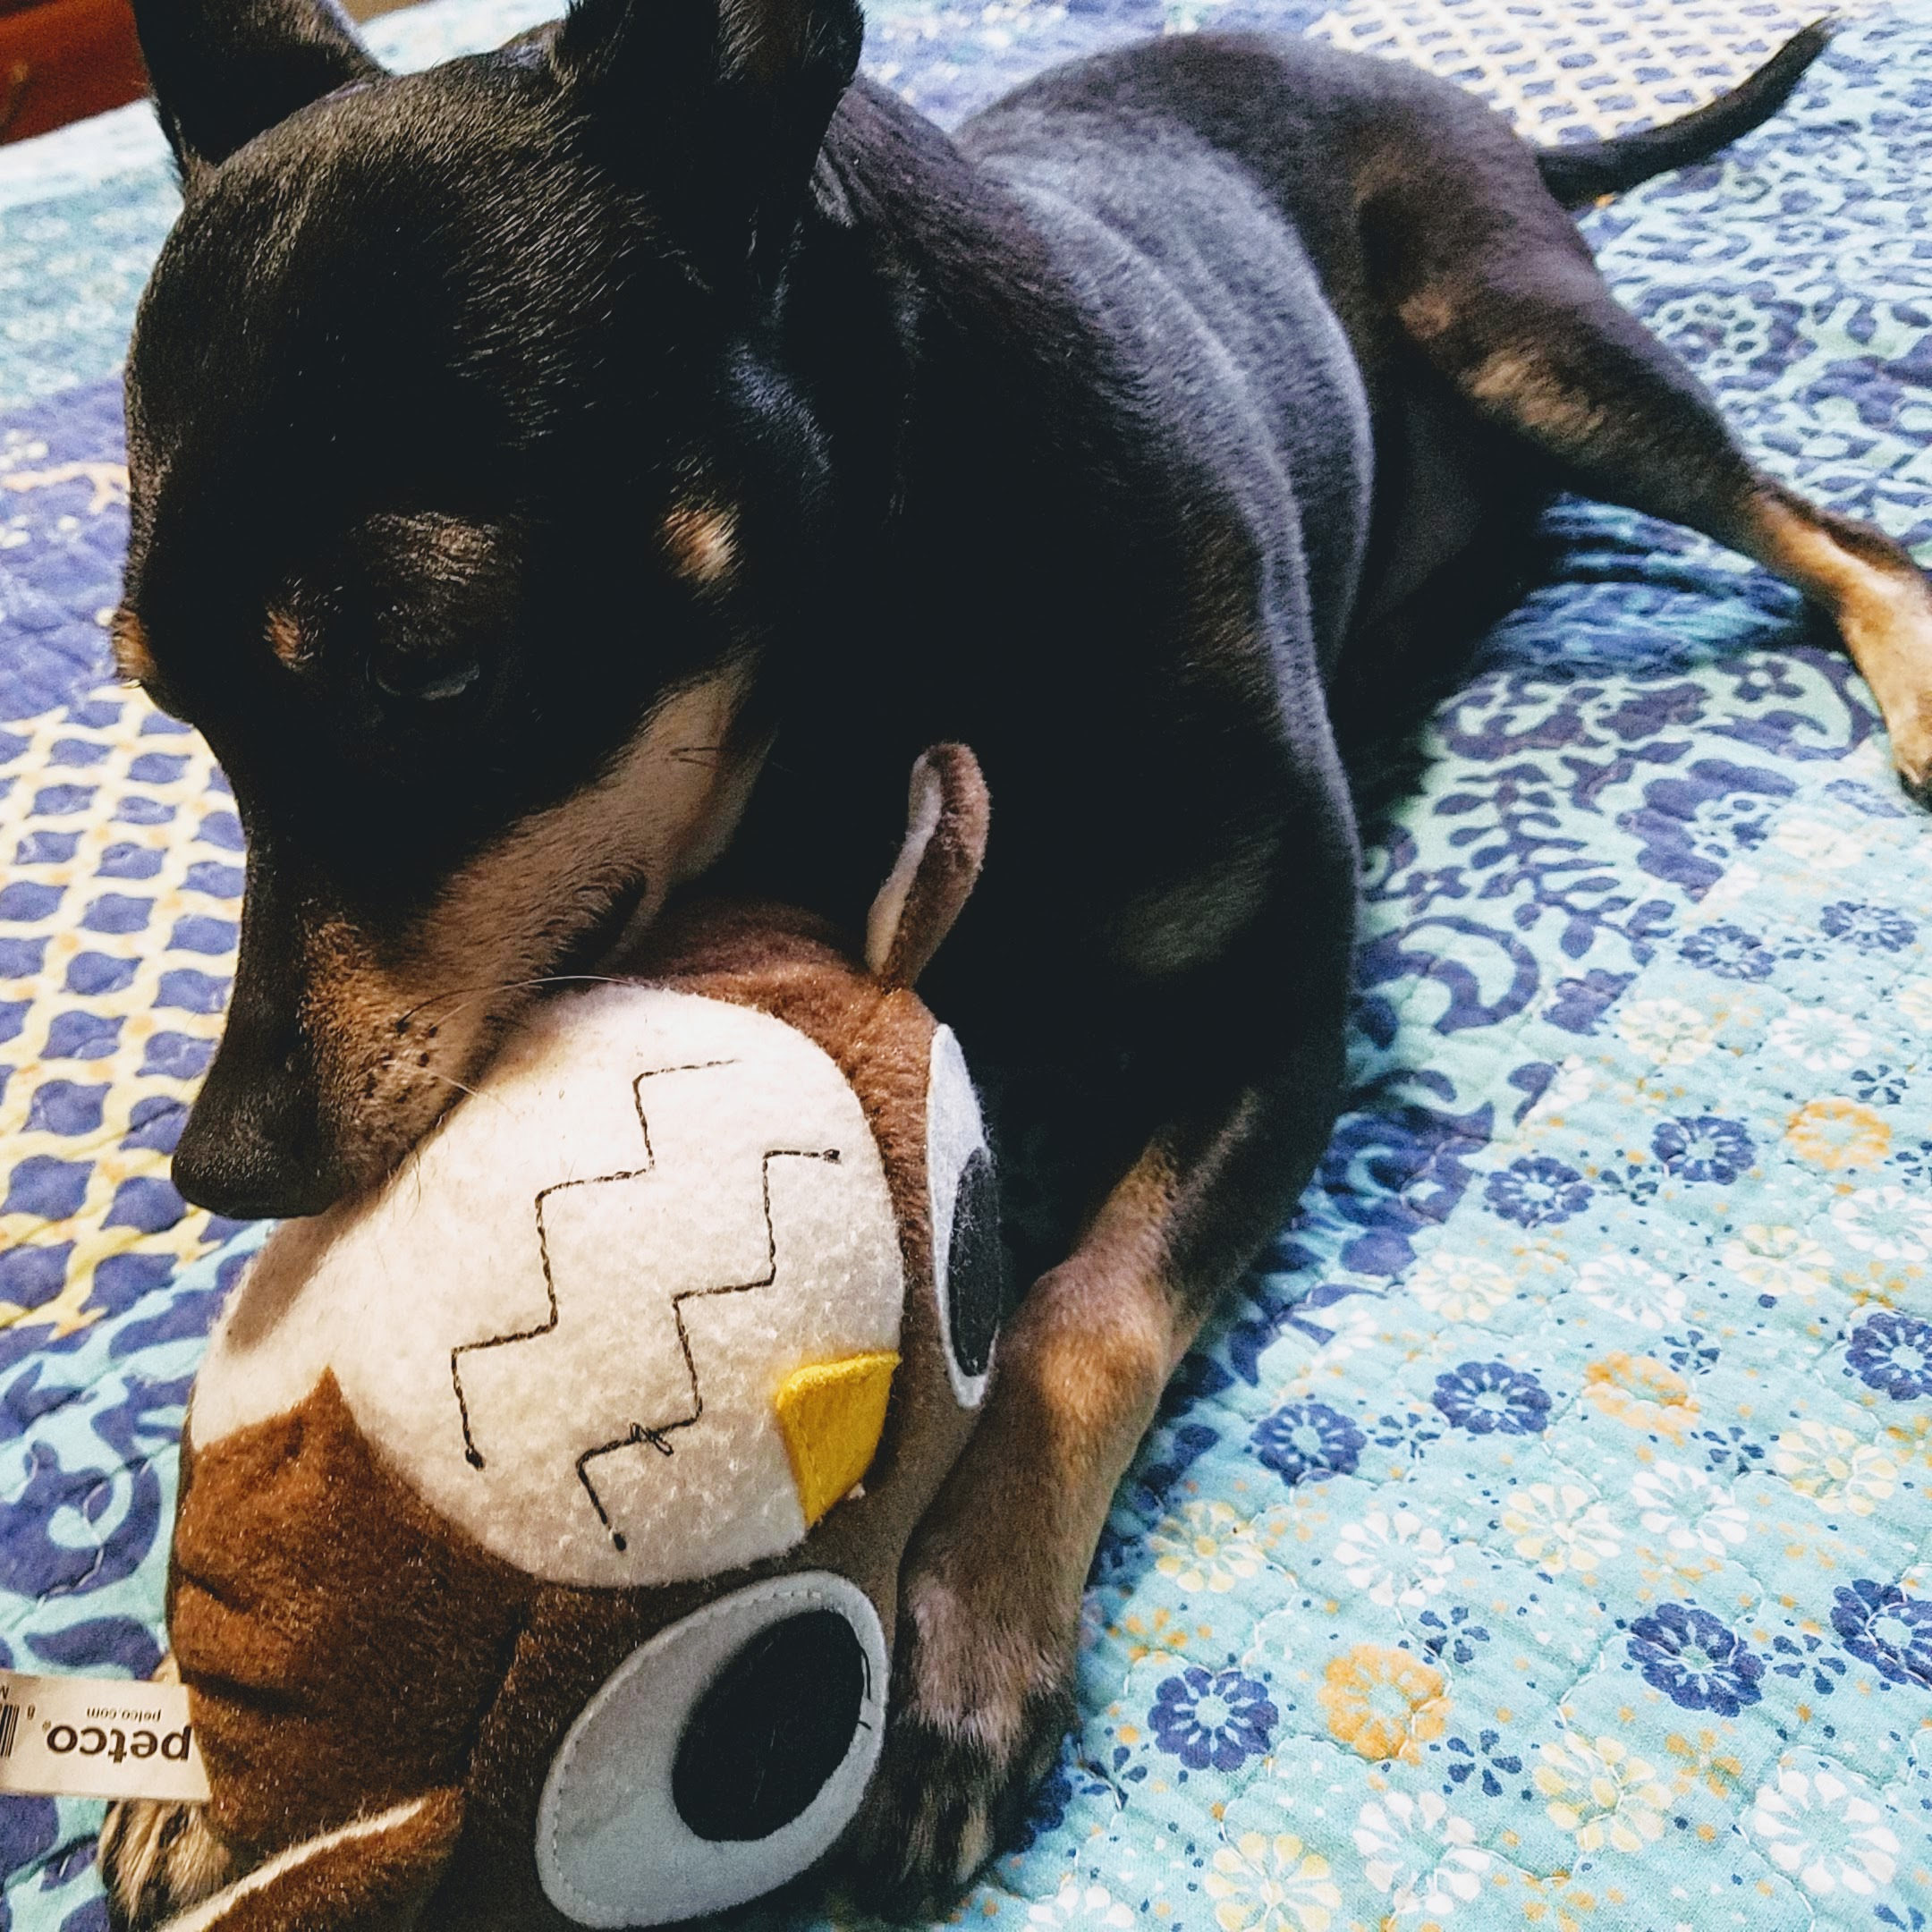
\includegraphics[width=2in]{../images/owl_Pepper}
			
			This less-than-wise owl missed the advice of avoiding the dog.
		\end{center}
	\end{block}	
\end{frame}


\begin{frame}{\fn}
	\begin{exercise}
		In the video for today we proved that the set $W=\{(a+b,3a,a-2b):a,b\in\R\}$ is a subspace of $\R^3$.
		
		In fact, this subspace is the plane $-2x+y-z=0$. 
		How do we show this? Notice that every vector in $W$ is on the plane because
			\[-2x+y-z=-2(a+b)+(3a)-(a-2b)=0.\]
		Think about the other hand. What $a$ and $b$ could we choose with respect to a point $(x,y,z)$ that satisfies $-2x+y-z=0$?
		That is, solve for $a$ and $b$ given the equation $(x,y,z)=(a+b,3a,a-2b)$, assuming $x$, $y$ and $z$ are fixed.
	\end{exercise}
\end{frame}
\begin{frame}{\fn}
	\begin{defn}
		The \emph{intersection} of two sets is the set consisting of everything that appears in both sets, the shaded region in the Venn diagram below.  The intersection of $V$ and $W$ is denoted $V\cap W=\{\vec x\ :\ \vec x\in V \text{ and }\vec x\in W\}$.
		\begin{center}
			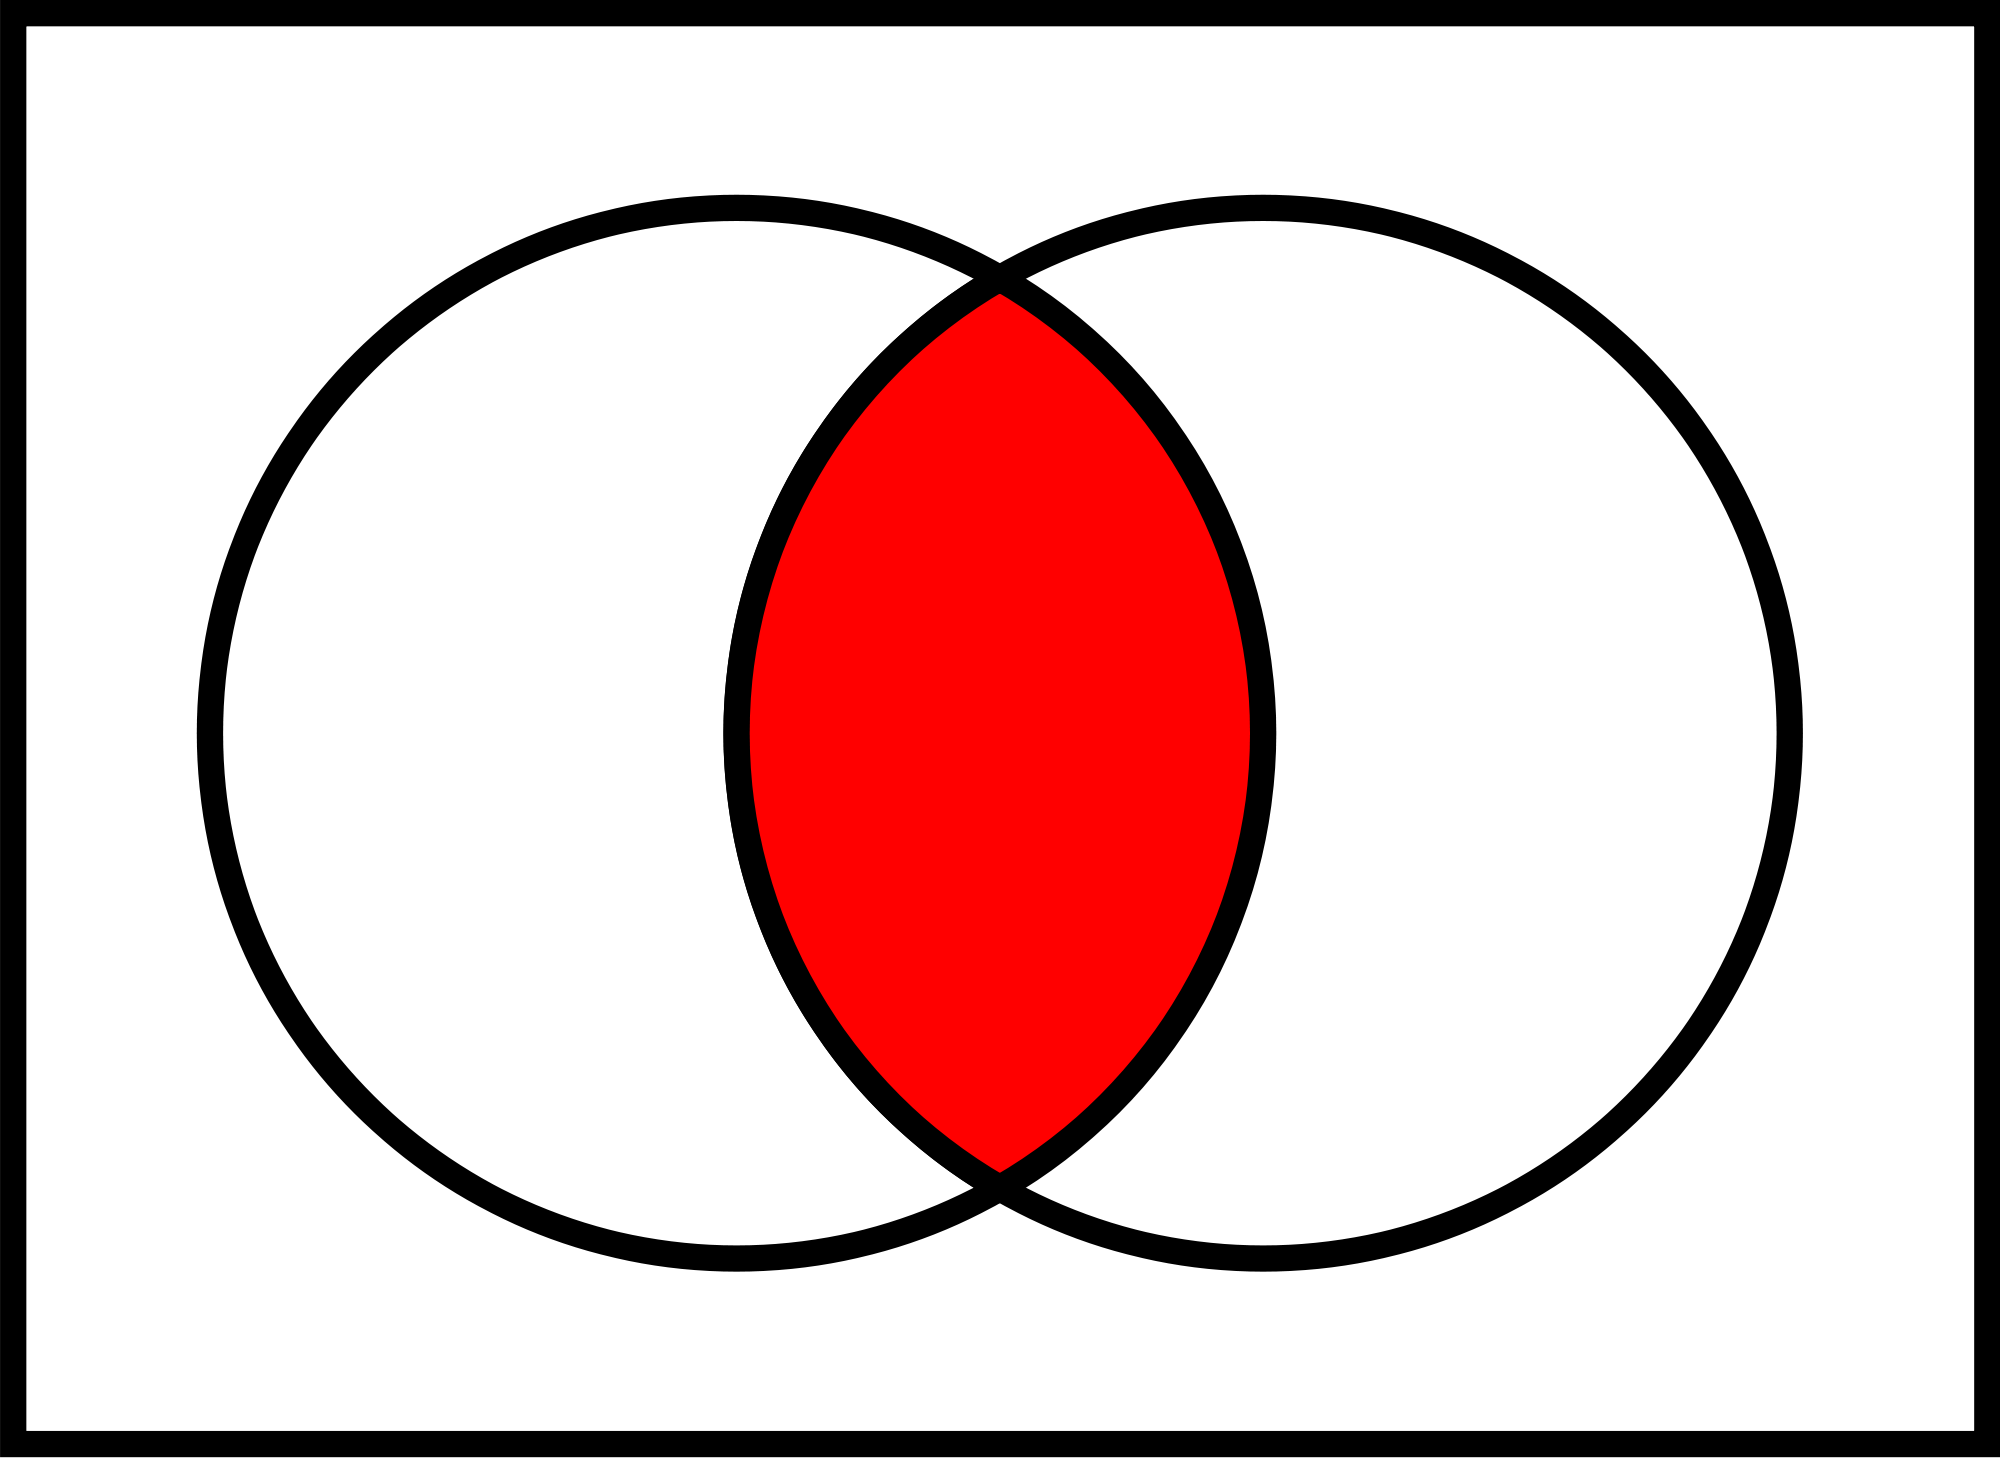
\includegraphics[width=1.5in]{../images/intersection}
		\end{center}
	\end{defn}
	\begin{statementblock}{Theorem 4.6}
		If $V$ and $W$ are both subspaces of a vector space $U$, then the {intersection} of $V$ and $W$ is also a subspace of $U$.
	\end{statementblock}
\end{frame}
\begin{frame}{\fn}
	\begin{exercise}
		Complete the proof of Theorem 4.6.
		\begin{proof}
			Let $V$ and $W$ be subspaces of a vector space $U$.  We want to show that $V\cap W$ is a subspace of $U$ using the subspace test.
			\begin{enumerate}[label=(\alph*)]
				\item Explain why $\vec 0\in V\cap W$.
				\item Let $\vec v$ and $\vec w$ be in $V\cap W$ this means that $\vec v$ and $\vec w$ are in $V$ and that $\vec v$ and $\vec w$ are in $W$.  Explain why $\vec v+\vec w$ is in $V\cap W$.
				\item Let $\vec v$ be in $V\cap W$ and $c$ be a scalar.  Explain why $c\vec v\in V\cap W$ too.
			\end{enumerate}
		\end{proof}
	\end{exercise}
\end{frame}
\begin{frame}{\fn}
	\begin{exercise}
		\begin{enumerate}[label=(\alph*)]
			\item Prove that the set $V=\{(a,b,a+b)\ :\ a,b\in\R\}$ is a subspace of $\R^3$.  
	
			\item Prove that the set $W=\{(a,b,3a)\ :\ a,b\in\R\}$ is a subspace of $\R^3$.
	
			\item Find the intersection of these sets and verify that it is also a subspace of $\R^3$. 
		\end{enumerate}
	\end{exercise}
\end{frame}
%\begin{frame}{\fn}
%	Just like in the case of $\R^n$ we can consider linear combinations for general vector spaces.
%	\begin{defn}
%		A vector $\vec v$ in a vector space $V$ is a \emph{linear combination} of $\vec u_1,\vec u_2,\dots,\vec u_n\in V$ if there exist scalars $c_1,c_2,\dots,c_n$ such that
%			\[\vec v=c_1\vec u_1+c_2\vec u_2+\cdots+c_n\vec u_n.\]
%	\end{defn}
%	\begin{exa}
%		The polynomial $p(x)=3+x-2x^2$ is a linear combination of $q_1(x)=1+x$, $q_2(x)=1+x^2$, $q_3(x)=1+x+x^2$, and $q_4(x)=x^2$ because \begin{eqnarray*}p(x)&=&3+x-2x^2\\ &=&5(1+x)+2(1+x^2)-4(1+x+x^2)+0x^2\\&=&5q_1(x)+2q_2(x)+(-4)q_3(x)+0q_4(x)\end{eqnarray*}
%	\end{exa}
%\end{frame}
%\begin{frame}{\fn}
%	\begin{exercise}
%			Can the polynomial $p(x)=1-4x+x^2$ be written as a linear combination of $q_1(x)=1+x$ and $q_2(x)=1+x^2$?
%	\end{exercise}
%	\begin{exercise}
%		Describe all of the polynomials can be written as a linear combination of $q_1(x)=1+x$ and $q_2(x)=1+x^2$.
%	\end{exercise}
%\end{frame}
\end{document}

